\thispagestyle{plain}
\section{Resolución de problemas con valores faltantes}
\boxabstract{Aprendizajes esperados}{Calcula valores faltantes en problemas de proporcionalidad directa,
    con constante natural, fracción o decimal (incluyendo tablas de variación).}

\subsection{Proporcionalidad directa y valor faltante}
\begin{boxK}
    \begin{center}\textbf{Inicio}\end{center}
    Menhir el arquitecto hizo un obelisco para conmemorar los setenta y seis años de su padre.
    Ahora hace un obelisco de menor tamaño, pero con la misma forma y del mismo material
    que el de su padre, para celebrar el decimonoveno cumpleaños de su hijo.
    \begin{enumerate}
        \item Las medidas de los obeliscos de Menhir están en la misma proporción que hay entre las
              edades de su padre y de su hijo. Si la altura del obelisco hecho en honor al padre es de
              12.2 m, ¿qué altura tiene el obelisco dedicado al hijo?

        \item Los obeliscos tienen base cuadrada. Si la base del obelisco dedicado al hijo tiene una
              longitud de 0.80 m por lado, ¿cuánto mide el lado de la base del obelisco más grande?
        \item Compartan sus respuestas y procedimientos con sus compañeros y escriban en su cuaderno
              el procedimiento que les parezca más acertado.
    \end{enumerate}
\end{boxK}

\begin{enumerate}
    \item En el local de jugos de Ana para preparar dos litros de agua de frutas se agregan,
          además de las frutas, cinco cucharadas de azúcar. Contesta lo siguiente
          \begin{enumerate}
              \item Si se mantiene la misma proporción, ¿cuántas cucharadas se necesitan para preparar ocho litros?
              \item Si agregó 33 cucharadas, ¿cuántos litros preparó?
              \item Si Ana utilizó 15 cucharadas, ¿cuántos litros prepararó?
              \item ¿Cuántas cucharadas se requieren para preparar un litro de agua?
          \end{enumerate}
    \item  Para llenar un vitrolero se necesitan cuatro litros de agua. Completa la tabla para
          saber cuántas cucharadas necesita Ana.
          \begin{figure}[H]
              \centering
              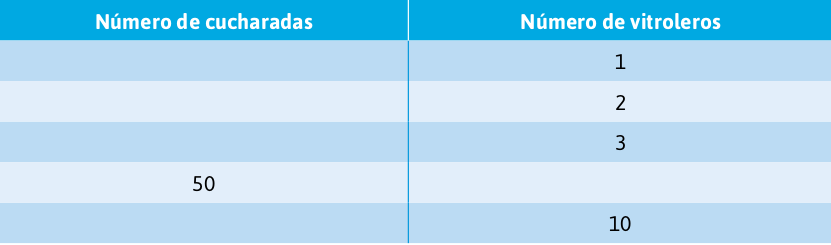
\includegraphics[width=0.6\linewidth]{tabla_vitrolero.png}
              \captionof{table}{}
              \label{tab:tabla_vitrolero}
          \end{figure}
          \begin{enumerate}
              \item ¿Cuántas cucharadas se necesitan para preparar un vitrolero?
              \item Si el número de vitroleros aumenta al doble, ¿cómo se incrementa el número de
                    cucharadas? ¿Y si aumenta al triple?
              \item Explica en tu cuaderno, cómo determinarías el número de cucharadas a partir del
                    número de vitroleros.
          \end{enumerate}

    \item Durante el Renacimiento, el estudio de la anatomía humana tuvo gran auge. Uno
          de los trabajos más conocidos es \emph{El hombre de Vitrubio} (ver figura \ref{fig:Hombre-de-Vitruvio}) de Leonardo
          da Vinci. Una de las proporciones más interesantes en esta obra es la relación entre
          la estatura de la figura y la distancia entre el ombligo y la base de los pies.

          \begin{minipage}{0.45\textwidth}
              \begin{figure}[H]
                  \centering
                  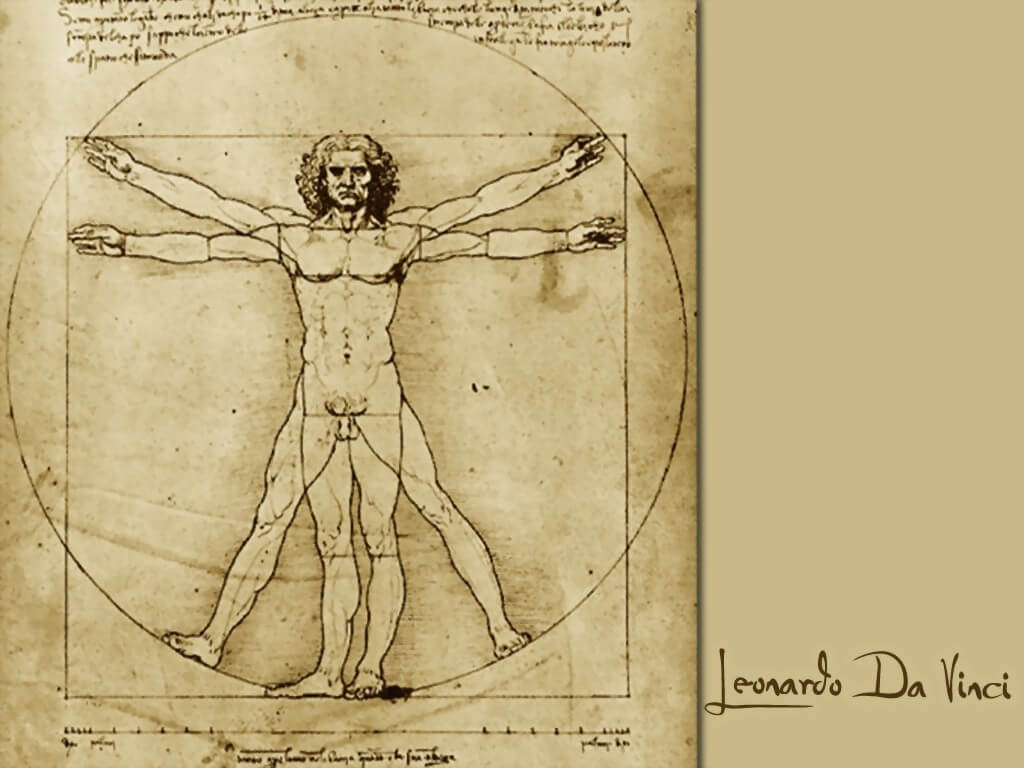
\includegraphics[width=\linewidth]{Hombre-de-Vitruvio.jpg}
                  \captionof{figure}{Obra de Leonardo Da Vinci, titulada \emph{El hombre de Vitrubio}}
                  \label{fig:Hombre-de-Vitruvio}
              \end{figure}
          \end{minipage}\hfill
          \begin{minipage}{0.45\textwidth}
              \begin{boxH}
                  Dos magnitudes tienen una relación de proporcionalidad directa si al aumentar o
                  disminuir una la otra aumenta o disminuye, respectivamente, en la misma proporción.
                  En este caso, al calcular la razón entre un valor de la primera magnitud y su correspondiente
                  de la otra magnitud, siempre obtendremos un número constante.
                  Si en una relación de proporcionalidad directa se desconoce un valor, se dice que
                  se trata de un problema de valor faltante.
              \end{boxH}
          \end{minipage}

          \begin{boxE}
              En \emph{El hombre de Vitrubio} se dice que la razón de su estatura respecto a la distancia
              del ombligo a los pies es perfecta y su valor es un número decimal no periódico e
              infinito: 1.61803\dots llamado \emph{proporción aúrea} (que redondeamos a 1.62).
          \end{boxE}

          \begin{enumerate}
              \begin{figure}[H]
                  \centering
                  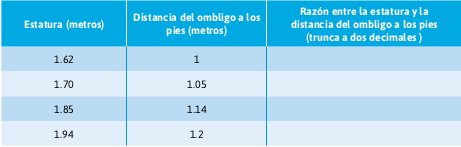
\includegraphics[width=0.6\linewidth]{tabla_hombre.png}
              \end{figure}
              \item Completa la tabla que relaciona la estatura de cuatro personas y la distancia de
                    su ombligo a sus pies.
              \item ¿Qué observas en la última columna?

          \end{enumerate}

    \item Contesta lo siguiente.
          \begin{enumerate}
              \item ¿Cuál es la estatura de Carlos si la distancia de su ombligo al piso es de 1.10 m?
              \item Si la estatura de María es 1.49 m, ¿Cuál es la distancia de su ombligo al piso?
              \item ¿Qué operaciones hicieron para resolver estos problemas?
          \end{enumerate}
\end{enumerate}

\begin{boxH}
    Si la razón entre dos datos correpondientes de dos conjuntos es siempre la misma,
    se dice que ese valor es una \textbf{constante de proporcionalidad}. En una relación de
    proporcionalidad directa al multiplicar los datos del segundo conjunto por la constante
    de proporcionalidad se obtienen los datos correspondientes del primer conjunto, y
    viceversa, multiplicando por el \textbf{\color{cyan}inverso multiplicativo} de esa constante.
\end{boxH}

\begin{boxH}
    \textbf{\color{cyan}Inverso multiplicativo.}
    El inverso multiplicativo de un número es aquel que al
    multiplicarlo por el primero da como resultado 1.
    Así, el inverso de 5 es $\dfrac{1}{5}$, porque $5\cdot \dfrac{1}{5}=1$
\end{boxH}

\begin{boxK}
    \begin{center}\textbf{Cierre}\end{center}
    Regresa al problema inicial, identifica una relación de proporcionalidad directa y calcula
    la constante de proporcionalidad.
    Revisa tus respuestas a los incisos $a$ y $b$ y valida el procedimiento del inciso $c$.
\end{boxK}
\newpage
\subsection{Proporcionalidad y valor unitario}

\begin{boxK}
    \begin{center}\textbf{Inicio}\end{center}
    Manolo y Sebastián compraron una bolsa con 100 canicas como la que se muestra en la
    figura, por \$80.00. Manolo aportó \$32.00 y Sebastián completó el pago.
    \begin{enumerate}
        \item ¿Cuánto pagó Sebastián?
        \item ¿Te parece justo que, al repartirlas, cada uno tenga 50 canicas? ¿Por qué?
        \item ¿Cuántas canicas debería recibir cada uno de acuerdo con lo que aportaron?
        \item Explica cómo decidiste repartir las canicas entre Manolo y Sebastián, y por qué
              consideras que de esa manera el reparto es justo.
    \end{enumerate}
\end{boxK}

\begin{enumerate}
    \begin{minipage}[t]{0.3\textwidth}
        \begin{figure}[H]
            \centering
            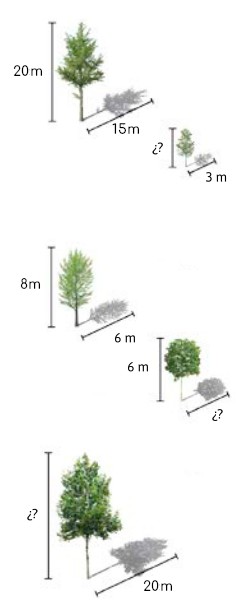
\includegraphics[width=\linewidth]{fig_sombras.png}
            \captionof{figure}{}
            \label{fig:fig_sombras}
        \end{figure}
    \end{minipage}\hfill
    \begin{minipage}[t]{0.65\textwidth}
        \item En un día soleado los objetos forman sombras y, a la misma hora, la altura y la
        sombra de diferentes objetos es proporcional.
        \begin{flushright}
            \begin{figure}[H]
                \centering
                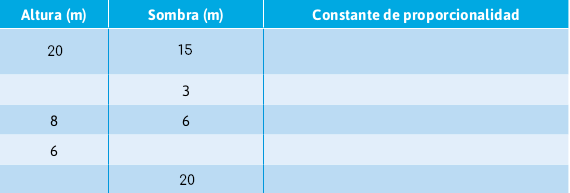
\includegraphics[width=0.85\linewidth]{tabla_sombras.png}
                \captionof{table}{}
                \label{tab:tabla_sombras}
            \end{figure}
        \end{flushright}
        \begin{enumerate}
            \item Con la información de la figura completa la tabla \ref{tab:tabla_sombras}.
            \item ¿Cómo son los números de la última columna?
            \item Si la sombra de un árbol mide 7.5 m, ¿cómo calcularías su altura? Explica.
            \item En primaria aprendiste a ubicar puntos en el plano cartesiano por medio de
                  coordenadas. Ubica los puntos cuyas coordenadas corresponden a la altura y sombra de los árboles
            \item La gráfica representa la relación entre la sombra y la altura de un árbol. Unan los
                  puntos que marcaron. ¿Qué observan?
        \end{enumerate}
    \end{minipage}

    \begin{figure}[H]
        \centering
        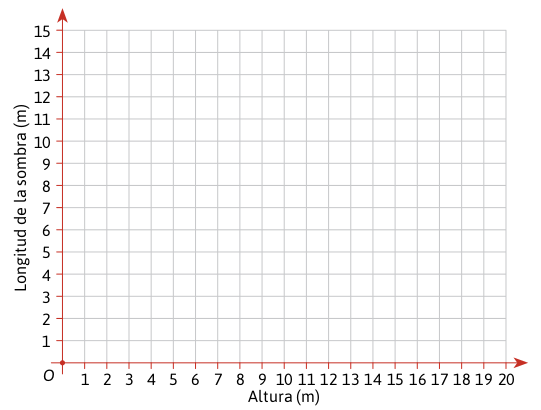
\includegraphics[width=.7\linewidth]{plano_sombras.png}
    \end{figure}

    \begin{figure}[H]
        \centering
        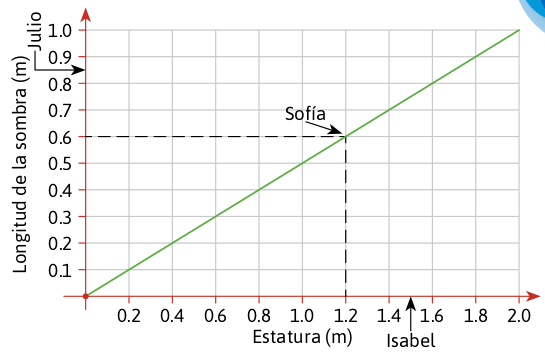
\includegraphics[width=0.6\linewidth]{graficas_sombras.png}
        \captionof{figure}{}
        \label{fig:graficas_sombras}
    \end{figure}

    \item La gráfica representa la relación entre la estatura de
          Sofía, Isabel y Julio y sus correspondientes sombras
          a las cuatro de la tarde de un día soleado. Obsérvenla y contesten.
          \begin{enumerate}
              \item Sofía mide 1.20 m y su sombra, 0.60 m. Si la estatura
                    de Isabel es 1.50 m, ¿cuánto mide la longitud de su sombra?
              \item La sombra de Julio tiene una longitud de 0.85 m. ¿Cuál es su estatura?
              \item Si Efrén, un amigo de Sofía, mide 1.84 m, ¿cuánto mediría su sombra?
              \item ¿Cuánto vale la constante de proporcionalidad entre la estatura de las personas y la longitud de su sombra?
              \item ¿Cuánto mide la sombra de un objeto cuya altura es de 1 m?
              \item Compara los resultados con los de tus compañeros y juntos describan cómo usar
                    la gráfica para obtener uno de los datos a partir del otro.
          \end{enumerate}

          \begin{boxH}
              Si dos o más razones tienen el mismo valor, entonces son \textbf{proporcionales}. El valor
              de esa razón corresponde a la \textbf{constante de proporcionalidad}.
          \end{boxH}

    \item Marca en la casilla las razones que forman una proporción.\\

          \begin{hoptboxes}
              \item $\dfrac{3}{4}   \text{ y } \dfrac{21}{28}$
              \item $\dfrac{32}{5}  \text{ y } \dfrac{96}{15}$
              \item $\dfrac{33}{42} \text{ y } \dfrac{17}{21}$
              \item $\dfrac{4}{5}   \text{ y } \dfrac{9}{12}$
              \item $\dfrac{1}{11}  \text{ y } \dfrac{3}{30}$
          \end{hoptboxes}

    \item La distancia que recorre un automóvil es proporcional al consumo de gasolina.
          Un automóvil recorre 180 km y gasta 12 L de gasolina.
          \begin{enumerate}
              \item ¿Cuántos kilómetros recorre con un litro?
              \item ¿Cuántos litros necesita para recorrer 480 km?
              \item ¿Cuál es el valor, en kilómetros, de la constante de proporcionalidad de la
                    distancia recorrida, por cada litro de gasolina consumido?
          \end{enumerate}
          \begin{boxH}
              En una relación de proporcionalidad el valor unitario es el valor de una de las
              magnitudes cuando el de la magnitud correspondiente es igual a 1; por ejemplo, los
              kilómetros que recorre un automóvil con 1 L de gasolina o el precio de un libro. El
              valor unitario es numéricamente igual a la constante de proporcionalidad.
          \end{boxH}
\end{enumerate}

\begin{boxK}
    \begin{center}\textbf{Cierre}\end{center}

    \begin{enumerate}
        \item A partir de lo que aprendiste en esta lección resuelve nuevamente el problema
              inicial. Verifica tus respuestas previas y compara tus procedimientos anteriores
              con los que aprendiste. ¿Ambos fueron correctos? ¿Cuál te parece más
              adecuado? ¿Por qué?
        \item Un tubo de 2 m de longitud pesa 16 kg. ¿Cuál será el peso de un tubo del mismo
              tipo, pero con 3 m de longitud?
    \end{enumerate}
\end{boxK}

\newpage

\subsection{Resolución de problemas de proporcionalidad directa}
\begin{boxK}
    \begin{center}\textbf{Inicio}\end{center}
    A Sofía y Pablo les tomaron una fotografía al lado de un árbol. Sofía sabe que su estatura es
    de 1.20 m y al medir con una regla su altura en la foto obtuvo 4 cm.
    \begin{enumerate}
        \item ¿Cómo obtendrías la estatura real de Pablo y la altura del árbol con base en la
              foto?
        \item Si en la fotografía el árbol mide 10 cm, ¿cuál es su altura?
        \item Si la altura real de Pablo es de 1.50 m, ¿cuánto mide su imagen en la fotografía?
        \item Escribe en tu cuaderno el procedimiento que seguiste.
        \item Compara tus resultados y procedimientos con los de tus compañeros. Argumenten la validez de los mis
    \end{enumerate}

\end{boxK}

\begin{enumerate}
    \item Las medidas de una plaqueta electrónica para teclado son de 32 cm por 24 cm. Si
          en una computadora se instalara una plaqueta, sin reducirla, el teclado mediría
          112 cm por 336 cm en vez de 14 cm por 42 cm que es lo usual.
          \begin{enumerate}
              \item ¿De qué tamaño deberán ser las plaquetas electrónicas para un teclado de tamaño común?
              \item ¿Cuánto se debe reducir la plaqueta grande para que sea del tamaño de una usual?
              \item Explica cómo obtuviste la respuesta, compara tu método con el de un compañero
                    y expongan al resto del grupo el método que les parezca más adecuado.
          \end{enumerate}

    \item La junta directiva de la secundaria Lázaro Cárdenas decidió que en las bibliotecas
          de aula haya 3 libros por cada cuatro alumnos.
          \begin{enumerate}
              \item Si en el salón de Edna hay 44 alumnos, ¿cuántos libros debe haber?
              \item Explica cómo determinaste el número de libros.
              \item Completa la siguiente tabla.
                    \begin{figure}[H]
                        \centering
                        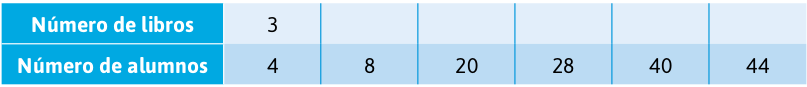
\includegraphics[width=0.6\linewidth]{tablaLibrosAlumnos.png}
                        \captionof{figure}{}
                        \label{fig:tablaLibrosAlumnos}
                    \end{figure}
              \item Escribe la constante de proporcionalidad que relacione el número de libros y el
                    número de alumnos.
          \end{enumerate}
    \item  Una tortuga avanza 48 cm en 12 segundos.
          \begin{enumerate}
              \item ¿Qué distancia recorrerá en un minuto si camina con la misma rapidez?
              \item Completa la siguiente tabla que Eduardo hizo para resolver el problem
                    \begin{figure}[H]
                        \centering
                        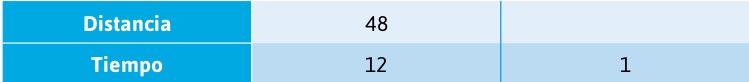
\includegraphics[width=0.6\linewidth]{tablaDistanciaTiempo.png}
                        \captionof{figure}{}
                        \label{fig:tablaDistanciaTiempo}
                    \end{figure}
              \item Eduardo escribió 4 en la casilla vacía, pero considera que está mal porque no es
                    posible que la tortuga en 1 min recorra menos distancia que en 12 s. ¿En qué
                    consiste su error?
              \item En tu cuaderno elabora una tabla como la de Eduardo, en el reglón de tiempo
                    incluye: una hora, un día y una semana. Escribe las distancias correspondientes
                    y comparte tus respuestas con el resto del grupo. Retoma la pregunta anterior y
                    explica en qué consistió el error de Eduardo.
          \end{enumerate}


    \item Si 4 toronjas se venden en 25 pesos, ¿cuánto cuestan 6 toronjas?
          \begin{enumerate}
              \item Completa la tabla con el valor que falta (valor faltante).
                    \begin{figure}[H]
                        \centering
                        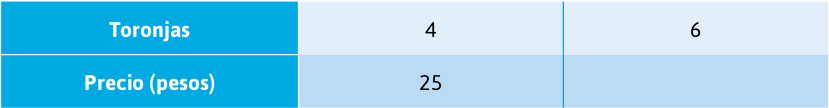
\includegraphics[width=0.6\linewidth]{tabla_toronjas.png}
                        \captionof{table}{}
                        \label{tab:tabla_toronjas}
                    \end{figure}
              \item Explica cómo obtuviste la respuesta.
              \item Completa la proporción a partir de los datos del problema y calcula el valor faltante.
                    \[\dfrac{25}{4} = \dfrac{}{6}\]
              \item ¿El valor faltante que propusiste en la tabla valida la igualdad anterior? Explica.
          \end{enumerate}
    \item Sofía leyó 25 páginas de un libro en 40 min. ¿Cuántas páginas leerá en 80 min si continua leyendo al mismo ritmo?
          \begin{enumerate}
              \item Escribe una proporción con un valor faltante para determinar cuántas páginas leerá en 65 minutos.
                    \[\dfrac{\text{ }}{\text{ }} = \dfrac{\text{ }}{\text{ }}\]
              \item Encuentra el valor faltante de la proporción anterior y verifica que se conserva la
                    igualdad de las razones.
              \item ¿Cuánto se consume la vela cada minuto?
              \item ¿En cuánto tiempo se consume 1 cm de vela?
              \item Completa la tabla.
                    \begin{figure}[H]
                        \centering
                        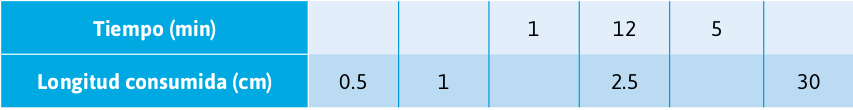
\includegraphics[width=0.6\linewidth]{tabla_longitud.png}
                        \captionof{table}{}
                        \label{tab:tabla_longitud}
                    \end{figure}
          \end{enumerate}

    \item Un avión Boeing 747 mide 77 m de largo por 63 de ancho (esta medida
          indica la longitud de las alas de un extremo al otro). Un modelo a escala
          mide 44 cm de largo.
          \begin{enumerate}
              \item ¿Cuál es el ancho del modelo a escala?
              \item Explica tu procedimiento para resolver el problema.
              \item ¿Cuánto debe medir la altura de una ventana en el modelo a escala si en el avión
                    real es de 0.7 m?
              \item ¿Cuál es la constante de proporcionalidad del modelo real al modelo a escala?
                    En este caso la constante recibe el nombre de \emph{escala del modelo}.
          \end{enumerate}

    \item Una receta para hacer dulce de membrillo indica que la cantidad de fruta debe
          ser una vez y media la cantidad de azúcar. Contesta.
          \begin{enumerate}
              \item Si se usan 2 kg de membrillo, ¿cuántos kilogramos de azúcar se necesitan?
              \item ¿Y si se usan 5 kg de membrillo?
              \item Completa la tabla e indica la constante de proporcionalidad que relaciona la cantidad
                    de membrillo y la cantidad de azúcar.
                    \begin{figure}[H]
                        \centering
                        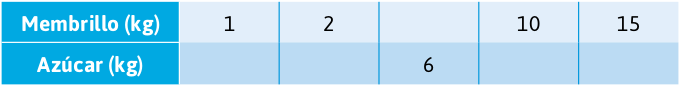
\includegraphics[width=0.6\linewidth]{tabla_azucar.png}
                        \captionof{table}{}
                        \label{tab:tabla_azucar}
                    \end{figure}
              \item Si la cantidad de membrillo aumenta ocho veces, ¿cuánto aumentará la cantidad
                    de azúcar?
              \item Si la cantidad de membrillo disminuye a la mitad, ¿cómo cambiará la cantidad de
                    azúcar?
          \end{enumerate}
    \item Un tren tarda 40 min en recorrer 130 km. ¿Cuánto tardará en recorrer 195 km si
          mantiene la misma rapidez? Explica tu procedimiento.
    \item Al medir el ritmo cardiaco de un paciente, durante 5 s el médico le dijo: \emph{su
              pulso está bien, usted tiene 72 pulsaciones por minuto}.
          \begin{enumerate}
              \item ¿Qué cálculo piensas que hizo el médico para saber el número de pulsaciones
                    por minuto si sólo tomó el pulso por 5 segundos?
          \end{enumerate}
    \item Para hacer mermelada de fresa se necesitan 3 kg de fresas frescas por cada 2 kg
          de azúcar. Karol sólo tiene 2.5 kg de fresas. Contesta.
          \begin{enumerate}
              \item ¿Cuánta azúcar debe utilizar para que el sabor de la mermelada sea el mismo que
                    el de la receta original?
              \item Explica el procedimiento que seguiste para resolver el problema.
              \item Si Antonio tiene 3.6 kg de azúcar, ¿cuántos kilogramos de fresas necesita si quiere emplear toda la azúcar?
              \item Explica tu procedimiento para resolver el problema.
              \item Alejandro cuenta con $\dfrac{3}{4}$ kg de fresas. ¿Cuántos kilogramos de azúcar debe emplear?
          \end{enumerate}
    \item Una bomba mueve 300 L de agua por hora. ¿Cuánto tardará en llenar un depósito de 3 200 litros?
    \item Una compañía envasadora necesita comprar una máquina que lave al menos 900
          botellas en 1 hora.
          \begin{enumerate}
              \item El vendedor les muestra una máquina que lava 60 botellas en 5 min. ¿Esta máquina cumple con los requerimientos de la compañía? ¿Por qué?
              \item El instructivo de otra máquina muestra la gráfica de
                    la figura \ref{fig:tabla_instructivo}. ¿Esta máquina cumple las necesidades de la compañía? ¿Por qué?

              \item ¿Cuál de las dos máquinas lava más botellas por unidad de tiempo?
                    \begin{figure}[H]
                        \centering
                        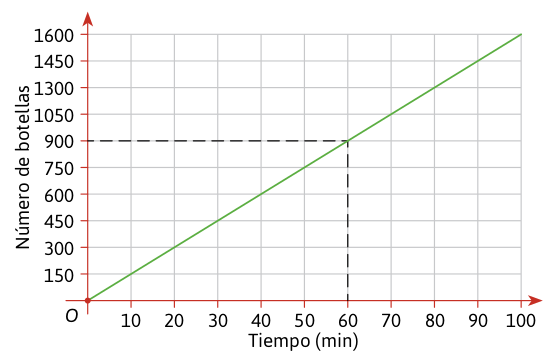
\includegraphics[width=0.5\linewidth]{tabla_instructivo.png}
                        \captionof{figure}{}
                        \label{fig:tabla_instructivo}
                    \end{figure}

          \end{enumerate}
\end{enumerate}

\begin{boxK}
    \begin{center}\textbf{Cierre}\end{center}

    \begin{enumerate}
        \item Retoma el problema de la sección Inicio y verifica tus respuestas.
              \begin{enumerate}
                  \item ¿Cuál es la constante de proporcionalidad que relaciona las medidas de los
                        objetos reales con los de la fotografía?
              \end{enumerate}
        \item ¿Cómo verificarías sin dividir la proporción $\dfrac{7.5}{1.5} = \dfrac{15}{3}$?
        \item Encuentra el valor faltante en las siguientes proporciones.\\

              \begin{hoptions}
                  \item $\dfrac{}{25} = \dfrac{32}{8} $
                  \item $\dfrac{25}{25} = \dfrac{}{10}$
                  \item $\dfrac{30}{} = \dfrac{54}{9} $
              \end{hoptions}
    \end{enumerate}
\end{boxK}

\begin{boxH}
    ¿El perímetro de un cuadrado es proporcional a las medidas de sus lados?
    Explica.\\
    Si las medidas de un rectángulo se duplican, ¿el área del nuevo rectángulo
    también se duplica respecto al inicial? Justifica tu respuesta.
\end{boxH}

\newpage